\documentclass[12pt,a4paper]{article}
\usepackage[utf8]{inputenc}
\usepackage[margin=1in]{geometry}
\usepackage{graphicx}
\usepackage{amsmath}
\usepackage{amsfonts}
\usepackage{enumerate}
\usepackage{listings}

\lstset{
    basicstyle=\ttfamily\small, % Font style and size
    numbers=left,               % Line numbers on the left
    numberstyle=\tiny,          % Line number style
    frame=single,               % Frame around the code
    breaklines=true,            % Allow line breaking
    captionpos=b                % Caption position (b for below)
}

% Title and Author
\title{TMA4162 Computational algebra, Project 1}
\author{Andreas Moe}
\date{\today}

\begin{document}

\maketitle

\section*{Introduction}
This report provides an overview of a topic studied in school. The goal of this document is to summarize key points, explain findings, and draw relevant conclusions.

\section*{Task 1}
Code implementing the arithmetic for the group \(\mathbb{F}_p^*\) can be found in the appendix.

\section*{Task 2}

\begin{enumerate}[a)]
    \item Code for exponentiation and unit tests can be found in the appendix.
    \item 
\[{T_{naive}}(a, p_{size}) = a*M(p) = O(exp(a_{size})*M(p_{size}))\]
\[{T_{squaremultiply}}(a, p_{size}) = {T_{squaremultiply}}(a/2, p_{size})+0.5*M(p_{size}))\]
\[= O(log_2(a))*O(M(p_{size}))=O(a_{size}*M(p_{size}))\]

    \item Figure 1 shows log(run time) vs the size of the prime for both algorithms. There is a clear exponential relationship between run time and prime size for the naïve algorithm, which is consistent with the theoretical result. The results for square and multiply do not seem to be inconsistent with the theory.
\end{enumerate}

\begin{figure}[htbp]
    \centering
    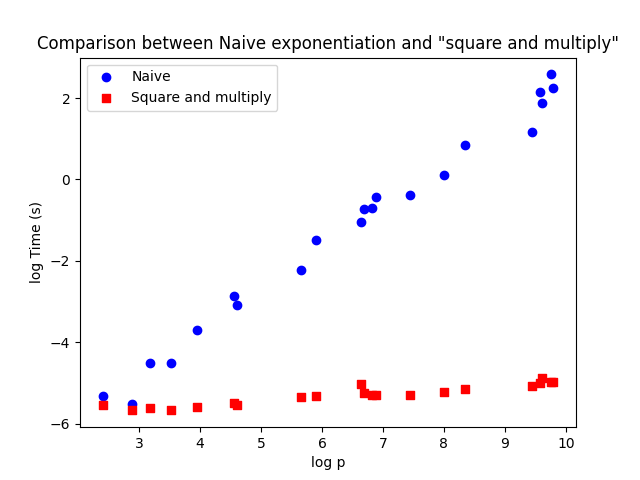
\includegraphics[width=\linewidth]{plot_2025-01-24 14-39-00_0.png}
    \caption{Measurements}
    \label{figure1}
\end{figure}
\newpage
\begin{appendix}
\section*{Appendix}
    Code is available at https://github.com/andrmoe/ComputationalAlgebra
    \lstinputlisting[language=Python, caption={algorithms}, label={lst:python_code}]{assignment1.py}
    \lstinputlisting[language=Python, caption={timing code}, label={lst:python_code}]{performance_test.py}
    \lstinputlisting[language=Python, caption={unit tests}, label={lst:python_code}]{test.py}
\end{appendix}

\end{document}
